\documentclass[conference]{IEEEtran}
\usepackage[T1]{fontenc}
\usepackage{graphicx}
\usepackage{url}
\usepackage{cite}
\usepackage{booktabs}
\usepackage{array}

\title{Locality versus Balance in Finite-Capacity Edge Caches}

\author{\IEEEauthorblockN{Author names to be finalized}
\IEEEauthorblockA{Affiliations and contact details to be supplied by the authors}}

\begin{document}
\maketitle

\begin{abstract}
Routing requests to a stable hash owner preserves cache locality, while
spreading requests can improve request-count balance but duplicate fills across
finite-capacity edge caches. We evaluate this trade-off in MiniCDN, a
single-host Docker prototype, using four seeded synthetic workloads and
consistent hashing, round robin, adaptive spillover, least-loaded router-local
routing, and a bounded-load router-local heuristic. In a retained
768-request comparison, consistent hashing achieved an 80.34\% HIT ratio on
Zipf demand, versus 76.69\% for adaptive routing; round robin achieved 65.49\%.
In a new 10-repetition sweep of 3,000 measured requests per trial, increasing
adaptive slack improved locality-sensitive outcomes: under Zipf demand, mean
HIT ratio rose from 74.74\% at slack 0 to 90.87\% at slack 1000, while excess
origin attempts fell from 523.5 to 39.8 per trial. Request-count coefficient
of variation rose over the same settings, exposing the balance/locality
trade-off. The effect was workload-dependent: the repeated-key cold-burst
workload required one origin attempt under consistent hashing and slack 1000
but three under several spillover settings. Per-request analysis did not
support a universal explanation that spilled requests cause higher tail
latency. One uniform/slack-1000 condition recorded 19 errors among 30,000
requests; its P95 is therefore reported with that caveat. Results are
descriptive of a closed-loop, single-host synthetic setup, not production CDN
performance.
\end{abstract}

\begin{IEEEkeywords}
content delivery networks, consistent hashing, caching, request routing,
finite cache capacity, load balancing
\end{IEEEkeywords}

\section{Introduction}
An edge cache's routing policy determines which requests share a cache.
Stable key ownership tends to concentrate each object's copies, preserving
effective capacity. A request-balanced policy can instead send the same key
to different edges, increasing duplicate fills and eviction pressure. Under
finite capacity, the policy trades off locality, balance, origin work, and
latency.

We ask: \emph{How does request-load-aware spillover change cache locality,
origin work, request-count balance, and client latency under finite edge-cache
capacity?} This work evaluates an experimental platform rather than proposing
a new hashing theorem or a production-ready CDN design. Contributions include
an instrumented benchmark; a repeated slack sweep with a distinct-key lower
bound on origin work; and a comparison with two explicitly router-local load
heuristics.

The results are mixed. For uniform and Zipf workloads, higher slack improves
HIT ratio and decreases excess origin attempts while increasing request-count
CV. The highest slack behaves much like consistent hashing on Zipf, while
several intermediate settings remain behind it. Cold-burst traces favor
keeping repeated keys together. Spill-latency results vary by workload and
cache status and do not establish a universal cold-edge penalty.

\section{Related Work}
Consistent hashing supports stable object assignment as server membership
changes; its foundational work also studies random cache trees for hot-spot
relief \cite{karger1997consistent}. Consistent hashing with bounded loads
formalizes a balance/movement trade-off for client-to-server assignments
\cite{mirrokni2018bounded}. These allocation-count guarantees do not directly
imply request-latency guarantees under nonuniform popularity or unequal
service costs. Later work addresses cascaded overflow with a minwise-hashing
approach \cite{chen2021revisiting}; our router-local heuristic is not an
implementation of either algorithm.

Cache-aware load balancing has been deployed for data-center search
applications, where a weighted voting scheme combines term locality with
replica selection \cite{archer2019cacheaware}. MiniCDN routes one HTTP
resource key per request and uses synthetic traces, so the mechanism and
evaluation are not directly comparable. Cache stampede prevention addresses
concurrent regeneration of expired objects \cite{vattani2015stampede};
MiniCDN fill coalescing is a distinct mechanism. HTTP conditional request
precedence follows RFC 9110 \cite{rfc9110}.

\section{System and Routing Policies}
MiniCDN comprises a router, three edge caches, an origin, and a Redis-backed
control service, run using Docker Compose. The edges use bounded body-byte
capacity and LRU replacement. Each experiment configures 64~KiB body capacity
per edge and 1~KiB origin objects; metadata and transient buffers are excluded.

The evaluated modes are consistent hash (route to hash owner), round robin,
adaptive spillover, least-loaded router-local, and bounded-load router-local.
Adaptive routing preserves the hash owner unless its router-local in-flight
reservation count exceeds the least-loaded candidate by more than configured
slack. The sweep uses slack values 0, 1, 2, 4, 8, and 1000; the final value
approximates pure hash for these runs. The bounded-load router-local mode uses
a local in-flight heuristic and capacity factor 2. It is not the theoretical
algorithm in \cite{mirrokni2018bounded}. Load state is not shared across
routers.

\section{Experimental Method}
\subsection{Configuration}
The main sweep uses uniform, Zipf (exponent 1.1), changing-hot-set, and
repeated-key cold-burst traces. Each trial has 256 warm-up requests, followed
by an acknowledged cache purge and 3,000 measured requests. Seeds derive
deterministically from base seed 2100260 plus run index. Each condition has
ten repetitions, concurrency is 16, cache TTL is one hour, and origin delay
is 20~ms. The environment is a single Docker host with closed-loop clients
and no network impairment.

The adaptive sweep covers six slack values across four workloads (240 trials).
A separate baseline sweep covers two router-local policies across four
workloads (80 trials). Together with the common routing-policy measurements,
the generated analysis has 400 trial rows.

\subsection{Metrics and Statistics}
HIT ratio is the fraction of requests reported as cache hits. For each
trial, the compulsory-miss floor is the number of distinct requested keys
after the cache reset; excess origin attempts equal actual origin attempts
minus this floor. Request-count coefficient of variation (CV) is computed
over the three edge counts. Per-request instrumentation records trial ID,
key, serving edge, hash owner, spill status, \texttt{X-Cache}, and client
latency.

HIT ratio, origin attempts, distinct-key floor, excess attempts, and request
CV use two-sided 95\% Student $t$-intervals over independent trial-level
values. P50/P95/P99 latencies and error counts use deterministic
10,000-resample percentile bootstrap intervals for the mean (seed 3102026).
Latency percentiles and spill groups are reduced per trial before inference;
individual requests are not treated as independent replicates.

\section{Results}
\subsection{Retained Comparison}
The retained October comparison is reproduced from
\texttt{routing-comparison.json} and \texttt{routing-requests.jsonl}. Its
Zipf HIT rates are 80.34\% (consistent hash), 65.49\% (round robin), and
76.69\% (adaptive); mean Zipf origin attempts are 151, 265, and 179.
Uniform HIT rates are 60.89\%, 21.09\%, and 48.44\%. Mean distinct-key
floors are 151.00 (Zipf), 176.33 (changing hot), 242.67 (uniform), and
1.00 (cold burst). Derived values are in
\texttt{routing-reproduction-2026-10-25.json} and
\texttt{routing-trials-derived-2026-10-25.csv}.

\subsection{Slack and Baseline Comparison}
In the extended sweep, uniform adaptive HIT ratio increases from 30.99\% at
slack 0 to 72.66\% at slack 1000, while excess attempts fall from 1814.2 to
567.0 per trial. For Zipf, HIT increases from 74.74\% to 90.87\%, and excess
attempts fall from 523.5 to 39.8. Zipf request CV rises from 0.084 to 0.313.
At slack 1000, Zipf closely matches consistent hashing: 90.88\% HIT, 39.4
excess attempts, and CV 0.313.

For Zipf at slack 2, adaptive records 83.70\% HIT, 254.9 excess attempts,
CV 0.184, and mean P95 76.6~ms. Consistent hash records 90.88\%, 39.4,
0.313, and 73.3~ms. Round robin records 73.02\%, 575.3, 0.000, and
106.2~ms. Least-loaded router-local records 75.00\%, 515.8, 0.090, and
97.8~ms. Bounded-load router-local records 87.88\%, 129.5, 0.268, and
85.0~ms. The values are means across ten trial-level replicates.

In cold burst, the per-trial distinct-key floor is one. Consistent hash and
adaptive slack 1000 average one origin attempt and 99.97\% HIT. Several
lower-slack settings average three origin attempts and 99.90\% HIT. Slack
1000 has CV 1.414, showing that preserving one repeated key can produce
uneven request counts.

One condition has nonzero errors: uniform adaptive slack 1000 recorded 19
errors among 30,000 requests. Its mean P95 is 176.2~ms with bootstrap 95\%
interval [62.4, 384.9]~ms. This condition is interpreted alongside the
errors and not as a reliable performance advantage. The trial summaries are
in \path{routing-analysis-2026-10-26-summary.csv}.

\subsection{Spill Latency}
For adaptive slack 2, spilled MISS P95 is higher than non-spilled MISS P95
for cold burst (39.0 vs.\ 35.0~ms), but lower for changing hot (91.0 vs.\
99.7~ms), uniform (92.0 vs.\ 93.1~ms), and Zipf (126.5 vs.\ 128.7~ms).
The results do not support a general claim that spilled requests explain
adaptive's higher tail latency. Spill status is observational, not a
randomized causal treatment. Trial-level confidence intervals are in the
spill-summary CSV.

\begin{figure}[t]
\centering
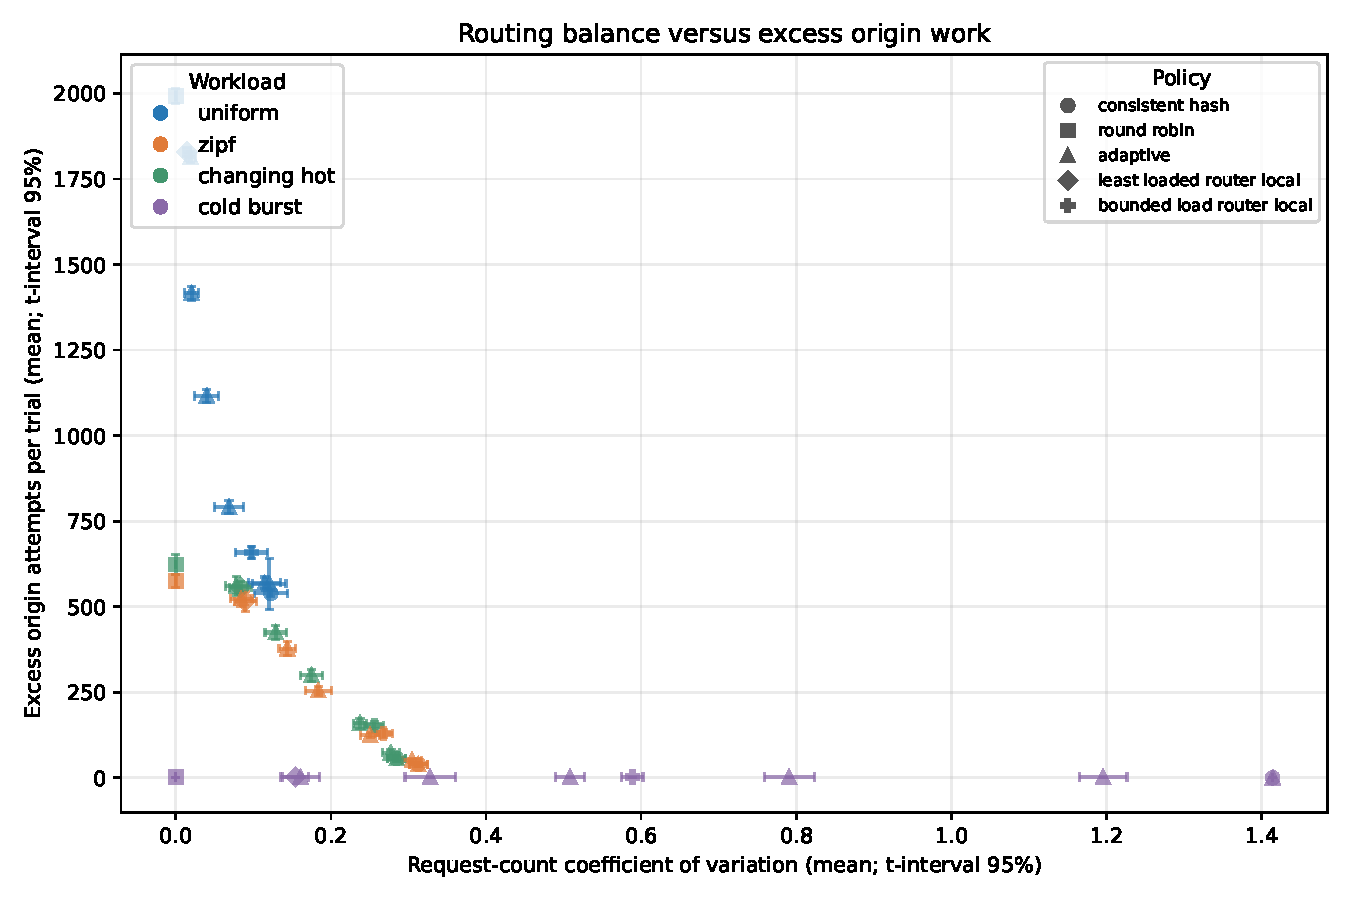
\includegraphics[width=\columnwidth]{../results/figures/routing-analysis-2026-10-26-pareto.pdf}
\caption{Excess origin attempts versus request-count CV. Points summarize
policy/workload conditions; error bars are trial-level 95\% $t$-intervals.}
\label{fig:pareto}
\end{figure}

\begin{figure}[t]
\centering
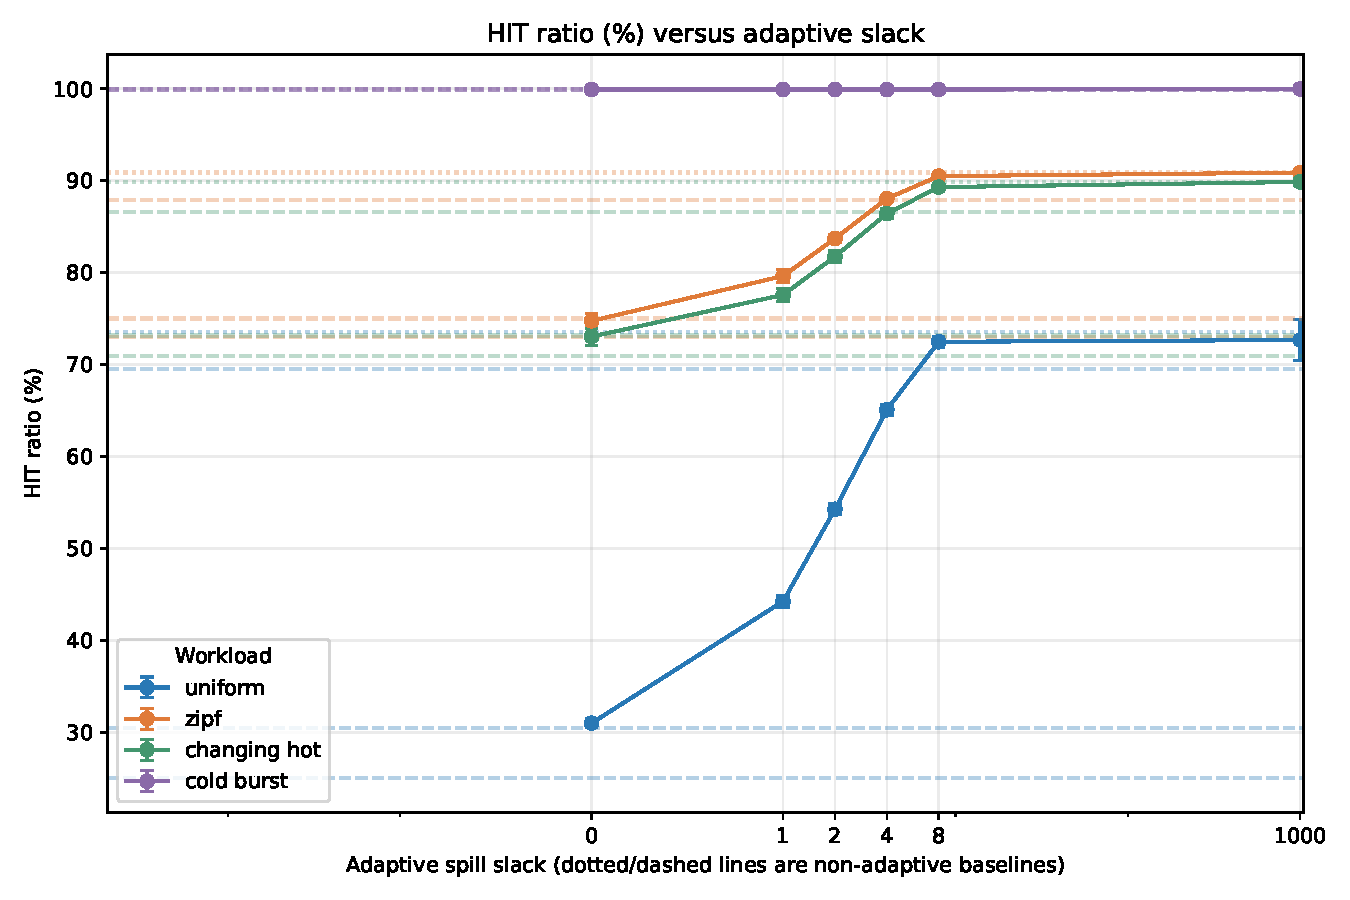
\includegraphics[width=\columnwidth]{../results/figures/routing-analysis-2026-10-26-hit-ratio.pdf}
\caption{HIT ratio versus adaptive spill slack. The plot includes non-adaptive
baseline reference lines.}
\label{fig:hit}
\end{figure}

\begin{figure}[t]
\centering
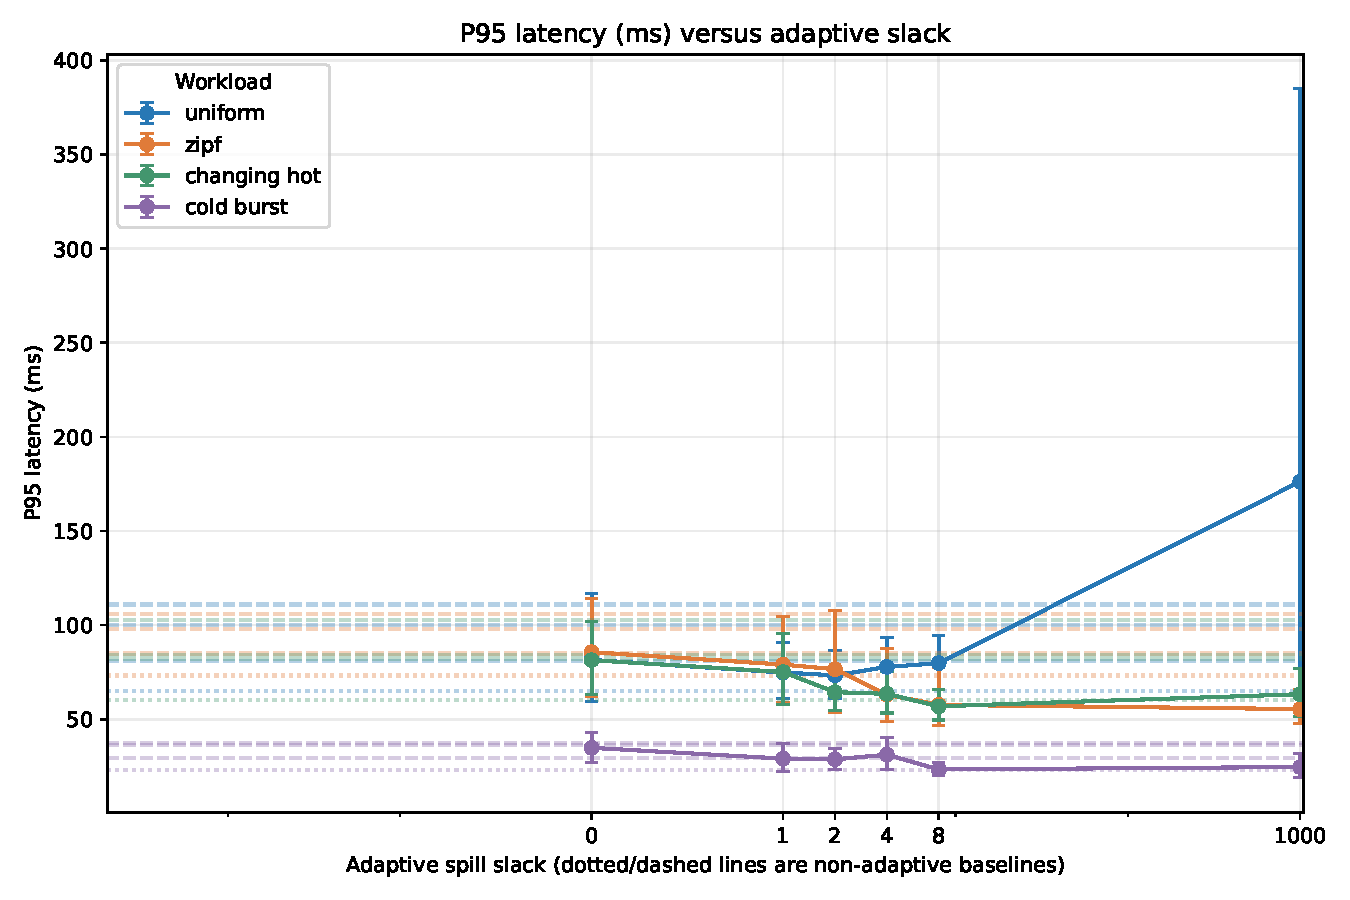
\includegraphics[width=\columnwidth]{../results/figures/routing-analysis-2026-10-26-p95.pdf}
\caption{P95 client latency versus adaptive spill slack. Error bars are
trial-level bootstrap 95\% intervals for the mean.}
\label{fig:p95}
\end{figure}

\begin{figure}[t]
\centering
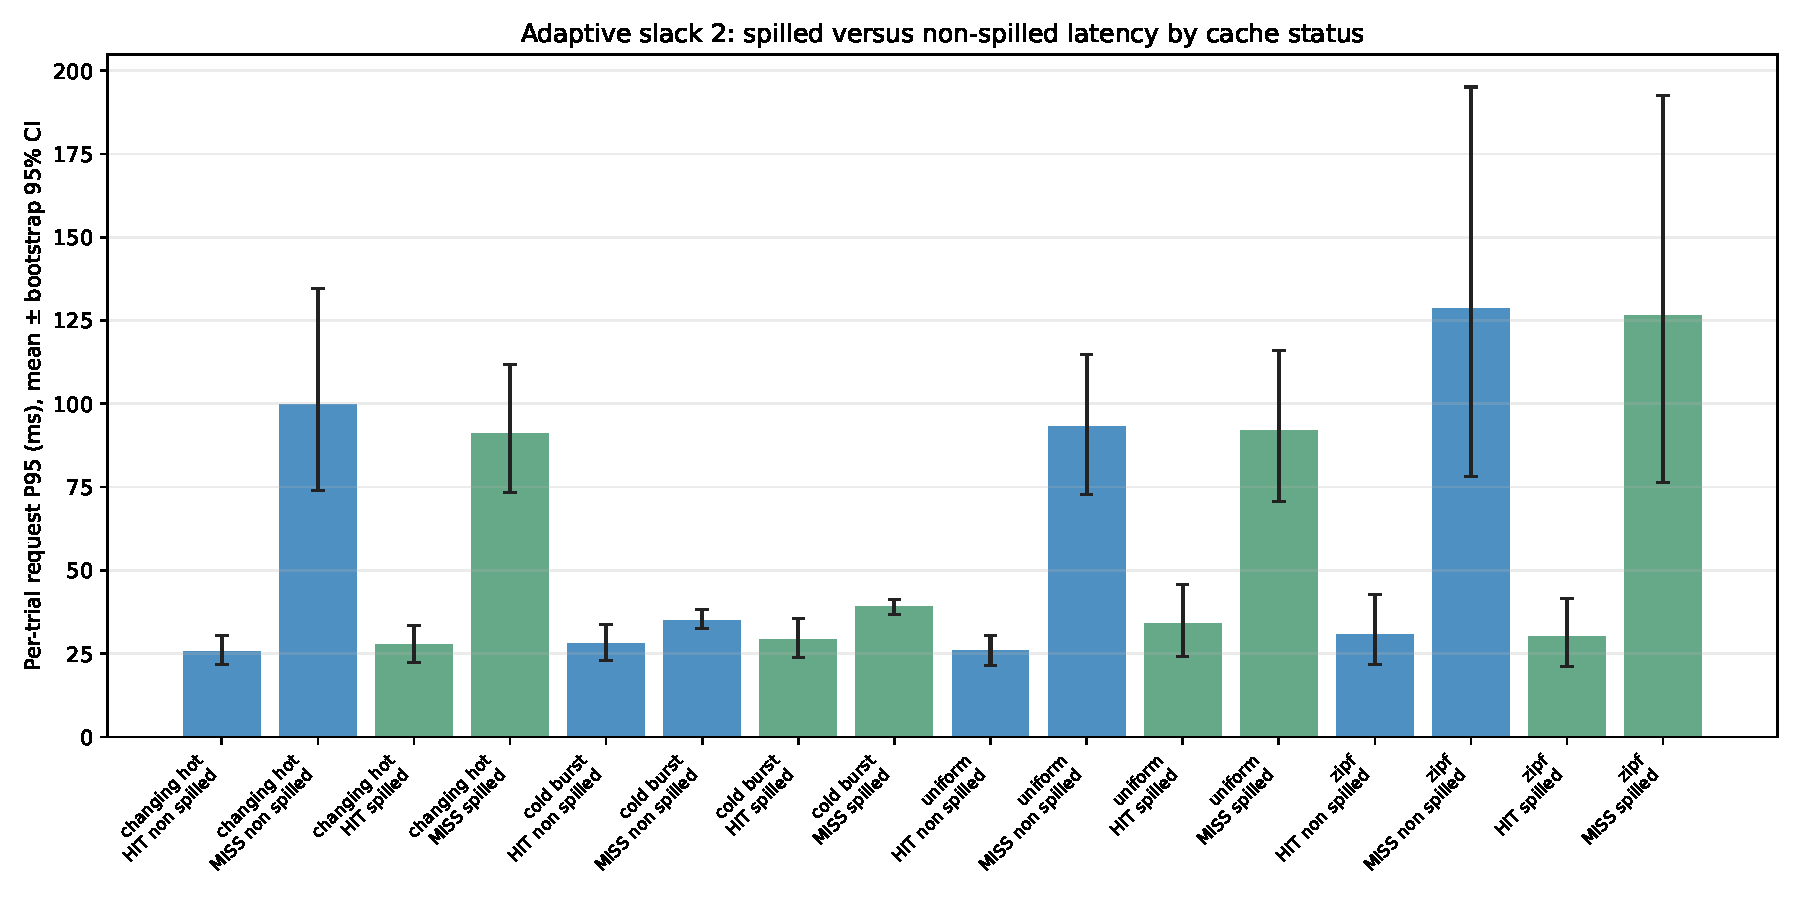
\includegraphics[width=\columnwidth]{../results/figures/routing-analysis-2026-10-26-spilled-latency.pdf}
\caption{Per-trial P95 latency for spilled and non-spilled requests, split by
workload and HIT/MISS status, at adaptive slack 2.}
\label{fig:spill}
\end{figure}

\section{Validator Correctness}
The origin handler follows RFC 9110 conditional-request precedence:
\texttt{If-None-Match}, when present, takes precedence over
\texttt{If-Modified-Since}. Tests exercise the real file handler and verify
that a mismatching ETag plus a future modification date returns 200, a
matching ETag returns 304, and \texttt{If-Modified-Since} alone can return
304. The tests are in \texttt{cmd/origin/main\_test.go}. The recorded full
Docker Go test run passed with 46.1\% total statement coverage.

\section{Discussion}
Increasing slack improves reuse and decreases excess origin work in uniform
and Zipf traces, but it also increases request-count CV. The evidence does
not establish that an adaptive load-aware policy outperforms consistent
hashing overall. Round robin balances request counts but pays more duplicate
origin work. The bounded-load router-local heuristic occupies an
implementation-specific intermediate point on some Zipf metrics; it is not
a theorem-backed bounded-load hash implementation.

Spill-latency results reject the initial simple explanation of a universal
cold-edge penalty. Because spill status was not randomized, this is
observational evidence and not a causal estimate.

\section{Threats to Validity}
The experiment uses one Docker host, a closed-loop client, synthetic traces,
three edge instances, and a synthetic fixed origin delay. It does not
establish behavior under open-loop arrivals, WAN latency, heterogeneous
edges, production request distributions, large objects, shared multi-router
load state, or changing membership. Router load state is local and
unshared. Four workload generators and one Zipf exponent limit
generalization. One condition contains 19 errors; its count and P95 are
disclosed, and the recorded evidence does not establish the cause. Ten
trial-level replicates per condition are not a substitute for independent
hosts. The distinct-key floor assumes a cold-start trace and does not model
prewarmed or externally shared caches. Cache capacity counts body bytes but
excludes metadata and runtime overhead.

\section{Conclusion}
The measured balance/locality trade-off is workload-dependent. In uniform
and Zipf traces, higher adaptive slack moves toward hash locality, improving
HIT ratio and reducing excess origin attempts while increasing request-count
imbalance. Round robin balances requests but incurs more duplicate origin
work. Consistent hashing is strong on locality-sensitive workloads, and
slack 1000 approximates it on Zipf. A repeated-key cold burst shows spillover
can turn one compulsory fill into multiple origin attempts. Per-request
evidence does not show spilled requests are universally slower, so high P95
must not be attributed to spillover without controlled causal experiments.

Future work should evaluate cache-size, origin-delay, and Zipf-exponent
sensitivity; repeat experiments on independent hosts with open-loop arrivals;
investigate the error-bearing condition; and compare with a faithful
bounded-load consistent-hashing implementation.

\section*{Data Availability}
All numerical results are derived from the dated JSON/CSV files under
\texttt{docs/academic/results/}. The retained source files are
\texttt{routing-comparison.json} and \texttt{routing-requests.jsonl}.
Analysis is generated with \texttt{scripts/analyze-routing-sweep.py}; trial
execution uses \texttt{scripts/compare-routing.mjs}. The command log and
remaining tasks are in \texttt{REPORT.md}.

\bibliographystyle{IEEEtran}
\bibliography{references}
\end{document}
